\documentclass[11pt,a4paper]{article}
\usepackage[T1]{fontenc}
\usepackage[utf8]{inputenc}
\usepackage{mathpazo}
\renewcommand{\ttdefault}{pcr}
\usepackage[english]{babel}
\usepackage[margin=2.3cm]{geometry}
\usepackage{microtype}
\usepackage{booktabs}
\usepackage{tabularx}
\usepackage{makecell}
\usepackage{graphicx}
\usepackage{float}
\usepackage{caption}
\usepackage{enumitem}
\usepackage{amsmath}
\usepackage{xcolor}
\usepackage[hidelinks]{hyperref}
\usepackage{xurl}

\captionsetup{font=small,labelfont=bf}
\setlist{itemsep=2pt,topsep=4pt}
\newcommand{\code}[1]{\texttt{#1}}
\renewcommand{\arraystretch}{1.12}

\title{\textbf{Assignment 3 --- Parallel Matrix Multiplication in Java}\\[4pt]
\large How the number of threads affects a shared-memory dense matrix multiplication}
\author{Pablo Martín Perdomo\\[2pt]
\small Big Data $\cdot$ Grado en Ciencia e Ingeniería de Datos $\cdot$ Universidad de Las Palmas de Gran Canaria}
\date{Assignment 3 $\cdot$ 13 November 2026}

\begin{document}
\sloppy
\maketitle

\begin{abstract}
\noindent We measured how the number of threads affects a shared-memory dense matrix multiplication in Java on a 6-core, 12-thread Intel Core i5-10400F. A sequential i-k-j kernel (the baseline) and a parallel version of the same kernel, which splits the rows of $C$ into contiguous chunks, were run on identical 64-bit matrices for $n = 250$ to $3000$ and 1 to 16 threads, in 3 independent JVM launches per configuration (7 repetitions each; medians of the launch medians reported). All 120 launches produced bit-identical results. For $n \ge 500$ the speedup is nearly ideal up to the 6 physical cores (efficiency 0.96--0.99). 12 threads give the shortest times for $n \ge 1000$ (largest speedup 6.79, $n = 2000$), but only 3--14\,\% faster than 6 threads; pinning two threads to one physical core showed that the second thread adds 4.7\,\% ($n = 1000$) and 15.5\,\% ($n = 2000$) of throughput, matching the measured gain from 6 to 12 threads. 16 threads (more than the logical processors) is 5--35\,\% slower than 12. An anomalous result of the first launch ($n = 1000$, 2 threads, $S = 1.63$) was traced, with a 35-launch follow-up, to JVM launches that run 16--26\,\% slower for their whole duration; over 3 launches the speedup is 2.00. The conclusions hold for this machine, this JVM and this kernel.
\end{abstract}

\section{Introduction and objective}

Multi-core CPUs make shared-memory parallelism the usual way to speed up dense linear algebra, but the gain depends on how the work is split, on the real execution resources of the hardware and on the problem size. This report is Assignment 3 of Big Data: a controlled study of parallel matrix multiplication in Java. It follows Assignment 1 (basic implementations) and Assignment 2 (optimised and sparse approaches, also in Java); here the best sequential kernel of Assignment 2 is executed in parallel.

\paragraph{Research question.} How does the number of threads affect the runtime of a Java shared-memory dense matrix multiplication on a 6-core, 12-thread desktop CPU, and for which matrix sizes and thread counts does parallel execution help?

\paragraph{Working hypotheses} (expectations drawn from the hardware description and standard parallel-performance background; Section~\ref{sec:hyp} compares them with the results):
\begin{itemize}
  \item[H1.] For large $n$, speedup is close to linear up to the number of physical cores (6).
  \item[H2.] Between 6 and 12 threads the extra threads share cores, so efficiency falls and speedup stays well below 12.
  \item[H3.] Using more threads than logical processors ($16 > 12$) brings no further gain.
  \item[H4.] For small $n$ the speedup saturates earlier, because each thread has less work.
  \item[H5.] The parallel implementation run with one thread is only slightly slower than the sequential baseline.
\end{itemize}

\section{Background and references}

\paragraph{Algorithm.} The kernel uses the i-k-j loop order over flat row-major arrays: for each row $i$ of $A$ and each $k$, the scalar $A[i][k]$ scales row $k$ of $B$ and is added to row $i$ of $C$. The inner loop walks $B$ and $C$ contiguously, which is cache-friendly. Every row of $C$ depends on one row of $A$ and on all of $B$, so rows can be computed independently: splitting them among threads needs no locks and no communication, and each thread receives almost the same amount of work.

\paragraph{Metrics.} Let $T_{\mathrm{seq}}(n)$ be the sequential time and $T_p(n)$ the parallel time with $p$ threads on the same input. Speedup is $S(p) = T_{\mathrm{seq}} / T_p$ and efficiency is $E(p) = S(p)/p$. Amdahl's law bounds $S(p)$ by the serial fraction of a program; Gustafson~\cite{gustafson}, re-evaluating that law, observes that this fraction depends on how the problem grows with $p$. Here the serial part (submitting tasks and waiting for them) is tiny, so Amdahl's bound is not expected to be the limiting factor; the hardware is.

\paragraph{Hardware limits.} The performance of matrix multiplication is governed by the memory hierarchy~\cite{goto}, and the Roofline model~\cite{roofline} bounds a kernel by either the peak arithmetic rate or the memory bandwidth times its arithmetic intensity. Hyper-Threading~\cite{marr} runs two logical processors on one physical core, sharing its execution units and caches, so a second thread on a core adds less than a whole core of throughput. This matters because the test CPU has 6 physical cores and 12 logical processors.

\section{Methodology}

\subsection{Implementations}

Both methods call the same kernel, use the same flat row-major \code{double[]} layout and read the same inputs; they differ only in how many rows one call processes.

\begin{table}[H]
\centering\small
\begin{tabularx}{\linewidth}{@{}lX@{}}
\toprule
Method & Description \\
\midrule
\code{ikj\_sequential} & One call over all $n$ rows (the baseline). \\
\code{ikj\_parallel} & The $n$ rows are split into $p$ contiguous chunks whose lengths differ by at most one row. Each chunk is one task on a fixed pool of $p$ threads (static scheduling). Every thread writes only its own rows of $C$, so no synchronisation on shared data is needed. \\
\bottomrule
\end{tabularx}
\end{table}

The thread pool is created and its threads are started before the first timed call. With $p = 1$ the parallel method still goes through the pool, so that run exposes the cost of the parallel machinery. No numerical library is used, so there are no internal library threads: the reported thread count is exactly the pool size. The kernel is the \code{ikj\_reorder} kernel of Assignment~2 (repository \code{Pancrasi0/Big-Data-Individual-Assignment-II}); it was checked to give bit-identical results to the Assignment~2 code for $n = 1$ to $300$, and the input generator to produce identical matrices for the same seeds.

\subsection{Inputs}

Matrix $A$ is generated with \code{java.util.Random} and seed 42, matrix $B$ with seed 43; values are uniform in $[1, 2)$ and stored as 64-bit floating point. Every configuration uses exactly the same matrices. Sizes: $n = 250$, 500, 1000, 2000 and 3000 ($n$ is the side of the square matrices).

\subsection{Environment}

\begin{table}[H]
\centering\small
\begin{tabularx}{\linewidth}{@{}lX@{}}
\toprule
Item & Value \\
\midrule
CPU & Intel Core i5-10400F @ 2.90\,GHz, 6 physical cores, 12 logical processors (logical CPUs $c$ and $c+6$ share physical core $c$, from \code{lscpu -e}) \\
RAM & 16,568,619,008 bytes (15.4 GiB) \\
Operating system & Linux 7.3.3-1-cachyos (CachyOS), amd64 \\
JVM & OpenJDK 64-Bit Server VM 21.0.12.1 (Arch Linux build), flags \code{-Xms4g -Xmx4g -XX:+UseParallelGC} \\
Compiler & \code{javac} with default flags \\
CPU frequency governor & performance \\
Thread affinity & none in the main study (the operating system schedules the threads); explicit with \code{taskset} in the pinned experiments (Section~\ref{sec:followup-method}) \\
Other load & no other applications running \\
Measurement date & 13 November 2026 (all experiments, in three sessions the same day) \\
\bottomrule
\end{tabularx}
\end{table}

\subsection{Correctness}

Every launch of the benchmark first runs 242 self-tests: a known $2\times2$ product, identity and zero matrices, random matrices ($n = 1$ to $129$) against an independent \code{double[][]} reference, bit-identity of the parallel result with the sequential one for 1, 2, 3 and 8 threads (including more threads than rows), and the row partitioning. Floating-point values are compared with $|x - y| \le 10^{-12} + 10^{-9}\cdot\max(|x|, |y|)$; different summation orders change rounding only by a few units in the last place, so the relative tolerance leaves a wide margin and still detects indexing errors. In the benchmark itself, every configuration's result is also verified with Freivalds' randomised test~\cite{freivalds} ($C\cdot x = A\cdot(B\cdot x)$ for two random vectors $x$) and summarised by a checksum of $C$.

\subsection{Measurement protocol}

\begin{itemize}
  \item \textbf{Timer and boundary.} \code{System.nanoTime} (monotonic). The timed region is one call of the multiplication. Inputs and the output array are created outside it; the zero-fill of $C$ is inside the kernel for both methods; task submission and waiting for the tasks are inside it for the parallel method. This boundary is the same in every comparison. The result is consumed through a checksum computed outside the timer.
  \item \textbf{Configurations.} A configuration is one size, one method and one thread count: 5 sizes $\times$ (1 sequential + 7 parallel thread counts: 1, 2, 4, 6, 8, 12 and 16), 40 configurations in total. 6 equals the physical cores, 12 the logical processors, and 16 oversubscribes the machine.
  \item \textbf{Launches and repetitions.} Every configuration was measured in 3 independent JVM launches. Each launch runs one configuration only, with 3 warm-up runs (recorded but excluded from the statistics) and 7 measured repetitions. Launch 1 is the original run of \code{scripts/run\_all.sh}. Launches 2 and 3 were added with \code{scripts/run\_rigor.py} later the same evening, with the same flags, inputs and protocol, one complete launch of all 40 configurations after the other. They were added because the follow-up of Section~\ref{sec:followup} showed that a whole JVM launch can run consistently slower than other launches of the same configuration. In total: 120 launches and 840 measured samples, all kept.
  \item \textbf{Statistics.} For each launch, the median and interquartile range (IQR $= Q_3 - Q_1$, linear interpolation) of its 7 repetitions. As the summary of a configuration we report the \emph{median of its 3 launch medians}, and as the spread between launches the \emph{range of the launch medians}. Speedup and efficiency use the summary medians. A launch is called \emph{slow} when its median exceeds the summary median of its configuration by more than 10\,\%.
  \item \textbf{Memory.} Three different quantities are reported: the estimated array storage ($3\cdot 8\cdot n^2$ bytes for $A$, $B$ and $C$), the live JVM heap after garbage collection, and the peak resident set size of the process (\code{VmHWM}), each as the median over the 3 launches. Because each launch runs one configuration, peak memory refers to a single configuration.
  \item \textbf{Budgets.} One multiplication may take at most 240\,s. The estimated storage is limited to 8192\,MB and, in the code, to 85\,\% of the maximum heap (about 3.5\,GB), which allows $n$ up to roughly 12,000. A timeout or memory failure would be recorded with its status and never given an invented time.
\end{itemize}

\subsection{Additional experiments}\label{sec:followup-method}

\paragraph{Follow-up for $n = 1000$.} Launch 1 produced one result that did not fit the others: $n = 1000$ with 2 threads took 329.37\,ms ($S = 1.63$, $E = 0.82$, against $E \approx 0.99$ for every other size). Because each configuration had then been measured in a single JVM launch, a follow-up (\code{scripts/run\_n1000.sh}) re-measured $n = 1000$ with the same protocol in 5 independent launches per configuration, interleaved so that consecutive launches are of different configurations:
\begin{itemize}
  \item \textbf{A, no affinity} (as in the main study): sequential, and parallel with 1, 2 and 4 threads.
  \item \textbf{B, pinned with \code{taskset}} (the whole JVM, including its JIT and GC threads, is restricted to the listed CPUs): parallel with 2 threads on two distinct physical cores (CPUs 0 and 1); parallel with 2 threads on the two logical processors of one physical core (CPUs 0 and 6); and parallel with 1 thread on CPU 0 as a reference.
\end{itemize}
This gives 35 launches and 245 measured samples. Its result motivated the extra launches 2 and 3 of the main study.

\paragraph{Hyper-Threading test for $n = 2000$.} To test directly whether two threads sharing a physical core explain the weak scaling above 6 threads, \code{scripts/run\_rigor.py} also ran, with $n = 2000$ and 3 launches each, the same three pinned placements as experiment B: 2 threads on CPUs 0 and 1, 2 threads on CPUs 0 and 6, and 1 thread on CPU 0.

\section{Results}

\subsection{Runtime}

Table~\ref{tab:runtime} gives the summary median of every configuration with the range of its launch medians, and Figure~\ref{fig:runtime} plots them. The shortest times are obtained with 12 threads for $n = 1000$, 2000 and 3000 (for $n = 3000$ the median falls from 18.34\,s sequential to 2.81\,s), with 6 threads for $n = 500$ (11.41\,ms) and with 16 threads for $n = 250$ (2.02\,ms, within the spread of 8 and 12 threads).

\begin{table}[htbp]
\centering\small
\caption{Median of the 3 launch medians, time per multiplication in ms; below it, in brackets, the range of the 3 launch medians (7 repetitions per launch).}\label{tab:runtime}
\setlength{\tabcolsep}{5pt}
\begin{tabular}{@{}lccccc@{}}
\toprule
Configuration & $n = 250$ & $n = 500$ & $n = 1000$ & $n = 2000$ & $n = 3000$ \\
\midrule
Sequential & \makecell{8.43\\ \scriptsize[8.43--8.58]} & \makecell{66.02\\ \scriptsize[66.01--66.80]} & \makecell{530.12\\ \scriptsize[528.88--537.45]} & \makecell{5354.17\\ \scriptsize[5349.36--5356.59]} & \makecell{18341.16\\ \scriptsize[18194.53--18757.64]} \\
Parallel, 1 thread & \makecell{8.56\\ \scriptsize[8.51--8.72]} & \makecell{66.53\\ \scriptsize[65.95--66.90]} & \makecell{557.51\\ \scriptsize[535.03--565.96]} & \makecell{5355.42\\ \scriptsize[5347.41--5494.10]} & \makecell{18854.49\\ \scriptsize[18195.97--18876.77]} \\
Parallel, 2 threads & \makecell{4.29\\ \scriptsize[4.26--4.33]} & \makecell{33.37\\ \scriptsize[33.32--33.38]} & \makecell{264.43\\ \scriptsize[264.14--329.37]} & \makecell{2692.35\\ \scriptsize[2688.86--2694.07]} & \makecell{9255.24\\ \scriptsize[9209.49--9296.87]} \\
Parallel, 4 threads & \makecell{2.19\\ \scriptsize[2.19--4.17]} & \makecell{16.80\\ \scriptsize[16.74--17.01]} & \makecell{134.98\\ \scriptsize[132.57--156.81]} & \makecell{1359.44\\ \scriptsize[1351.47--1360.67]} & \makecell{4623.57\\ \scriptsize[4614.35--4636.43]} \\
Parallel, 6 threads & \makecell{2.79\\ \scriptsize[1.49--2.81]} & \makecell{11.41\\ \scriptsize[11.27--13.36]} & \makecell{90.20\\ \scriptsize[88.50--113.98]} & \makecell{912.03\\ \scriptsize[907.95--937.46]} & \makecell{3097.16\\ \scriptsize[3089.30--3101.52]} \\
Parallel, 8 threads & \makecell{2.13\\ \scriptsize[2.12--2.14]} & \makecell{16.12\\ \scriptsize[16.10--16.20]} & \makecell{122.73\\ \scriptsize[119.85--126.44]} & \makecell{990.31\\ \scriptsize[984.48--1010.56]} & \makecell{3386.26\\ \scriptsize[3377.87--3410.62]} \\
Parallel, 12 threads & \makecell{2.14\\ \scriptsize[1.86--2.14]} & \makecell{12.16\\ \scriptsize[11.40--12.50]} & \makecell{87.65\\ \scriptsize[86.43--95.99]} & \makecell{788.44\\ \scriptsize[785.84--790.56]} & \makecell{2805.50\\ \scriptsize[2777.82--2819.17]} \\
Parallel, 16 threads & \makecell{2.02\\ \scriptsize[1.67--2.03]} & \makecell{12.80\\ \scriptsize[12.28--12.92]} & \makecell{96.75\\ \scriptsize[96.62--99.33]} & \makecell{886.66\\ \scriptsize[877.39--889.90]} & \makecell{3795.69\\ \scriptsize[3701.56--3844.48]} \\
\bottomrule
\end{tabular}
\end{table}

Inside a launch the variability is low: the IQR is below 1\,\% of the launch median in 76 of the 120 launches and below 5\,\% in 101. Between launches, the range of launch medians is at most 3.8\,\% of the summary for every configuration with $n \ge 2000$, but reaches 18--28\,\% for $n = 1000$ with 2, 4 and 6 threads and 47--90\,\% for $n = 250$ with 4 and 6 threads (Section~\ref{sec:launches}).

\begin{figure}[htbp]
\centering
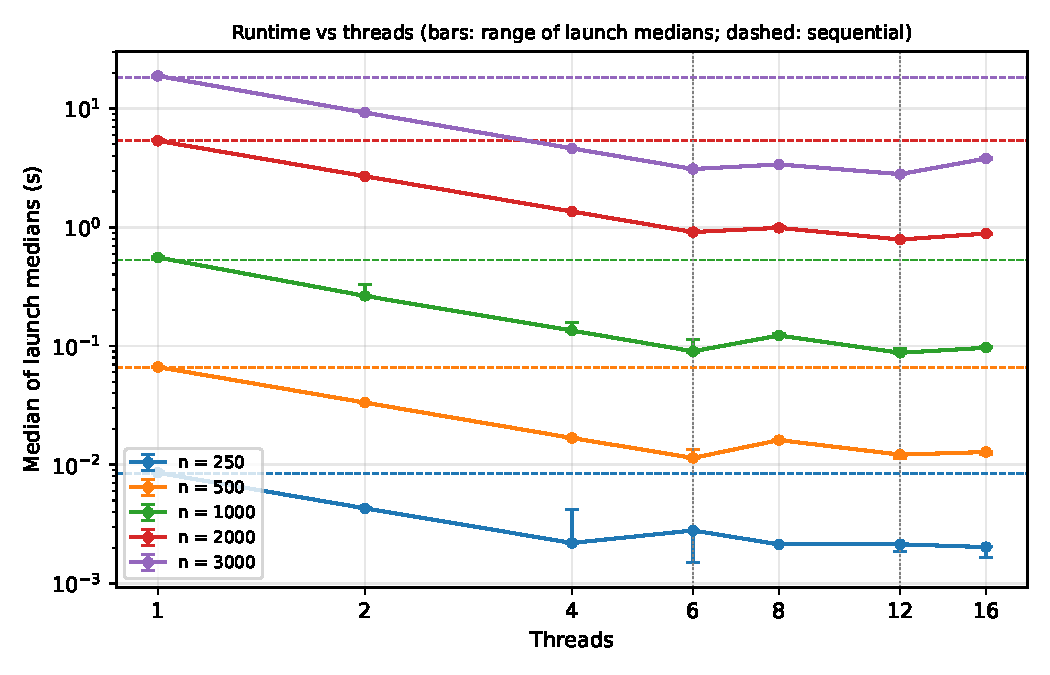
\includegraphics[width=0.8\linewidth]{figs/fig_runtime_launches.pdf}
\caption{Median of the 3 launch medians against the number of threads, log-log axes. Error bars: range of the launch medians; dashed horizontal lines: the sequential summary of the same colour; vertical lines: 6 physical cores and 12 logical processors.}\label{fig:runtime}
\end{figure}

\subsection{Speedup and efficiency}\label{sec:speedup}

\begin{table}[htbp]
\centering\small
\caption{Speedup $S(p)$ and, in parentheses, efficiency $E(p)$, computed from the summary medians of Table~\ref{tab:runtime} ($T_{\mathrm{seq}}$ is the sequential row).}\label{tab:speedup}
\begin{tabular}{@{}lrrrrr@{}}
\toprule
Threads $p$ & $n = 250$ & $n = 500$ & $n = 1000$ & $n = 2000$ & $n = 3000$ \\
\midrule
1 & 0.99 (0.99) & 0.99 (0.99) & 0.95 (0.95) & 1.00 (1.00) & 0.97 (0.97) \\
2 & 1.96 (0.98) & 1.98 (0.99) & 2.00 (1.00) & 1.99 (0.99) & 1.98 (0.99) \\
4 & 3.84 (0.96) & 3.93 (0.98) & 3.93 (0.98) & 3.94 (0.98) & 3.97 (0.99) \\
6 & 3.02 (0.50) & 5.79 (0.96) & 5.88 (0.98) & 5.87 (0.98) & 5.92 (0.99) \\
8 & 3.96 (0.49) & 4.09 (0.51) & 4.32 (0.54) & 5.41 (0.68) & 5.42 (0.68) \\
12 & 3.95 (0.33) & 5.43 (0.45) & 6.05 (0.50) & 6.79 (0.57) & 6.54 (0.54) \\
16 & 4.17 (0.26) & 5.16 (0.32) & 5.48 (0.34) & 6.04 (0.38) & 4.83 (0.30) \\
\bottomrule
\end{tabular}
\end{table}

Figures~\ref{fig:speedup} and~\ref{fig:eff} plot the same values. Observations, by thread count:
\begin{itemize}
  \item \textbf{2 and 4 threads:} the efficiency is between 0.96 and 1.00 for every size.
  \item \textbf{6 threads (the physical cores):} $E = 0.96$--$0.99$ for every size from $n = 500$ up. For $n = 250$, $E = 0.50$: two launches take about 2.8\,ms, slower than 4 threads, and the third 1.49\,ms.
  \item \textbf{8 threads:} $E = 0.49$--$0.68$ for every size, and slower than 6 threads by 41\,\%, 36\,\%, 9\,\% and 9\,\% for $n = 500$, 1000, 2000 and 3000.
  \item \textbf{12 threads (all logical processors):} the best median for $n \ge 1000$ ($S = 6.05$, 6.79 and 6.54, $E = 0.50$--$0.57$), but only 2.8\,\%, 13.6\,\% and 9.4\,\% faster than 6 threads. For $n = 500$, 12 threads is 6.6\,\% slower than 6 threads.
  \item \textbf{16 threads (oversubscription):} slower than 12 threads by 5\,\% ($n = 500$), 10\,\% ($n = 1000$), 12\,\% ($n = 2000$) and 35\,\% ($n = 3000$). For $n = 250$ it is 6\,\% faster, within the spread of those runs.
  \item \textbf{Smallest size:} for $n = 250$ the speedup stays between 3.95 and 4.17 for 8, 12 and 16 threads. The whole sequential multiplication takes only 8.4\,ms.
\end{itemize}

\begin{figure}[htbp]
\centering
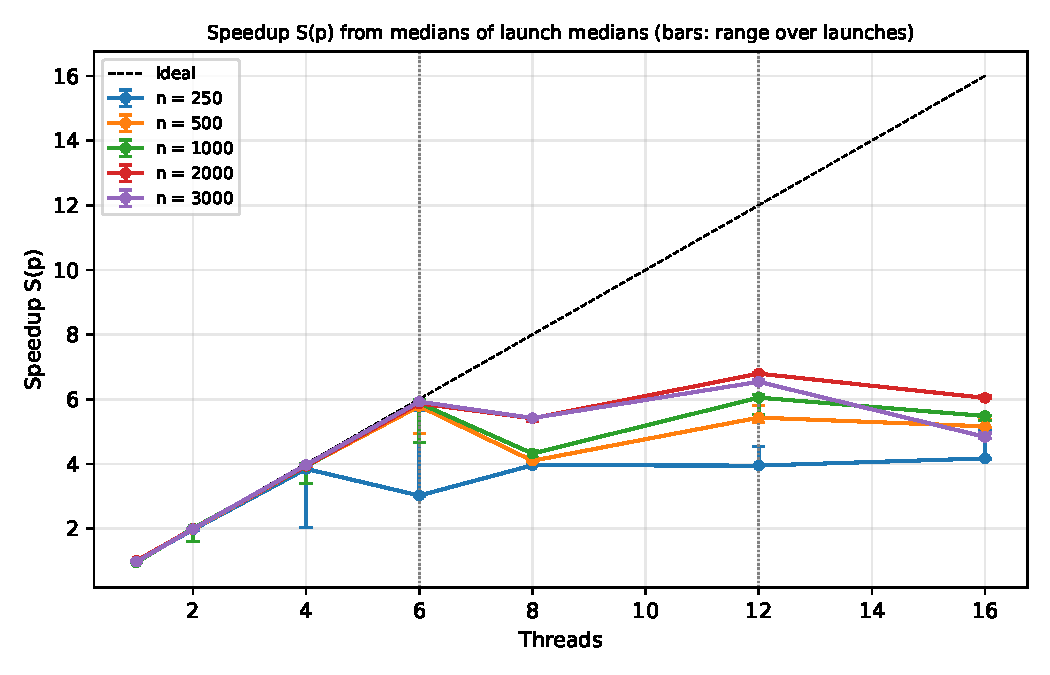
\includegraphics[width=0.75\linewidth]{figs/fig_speedup_launches.pdf}
\caption{Speedup $S(p) = T_{\mathrm{seq}}/T_p$ against the number of threads, from the summary medians, with the ideal $S(p) = p$. Bars: $T_{\mathrm{seq}}$ divided by the largest and by the smallest launch median of $T_p$.}\label{fig:speedup}
\end{figure}

\begin{figure}[htbp]
\centering
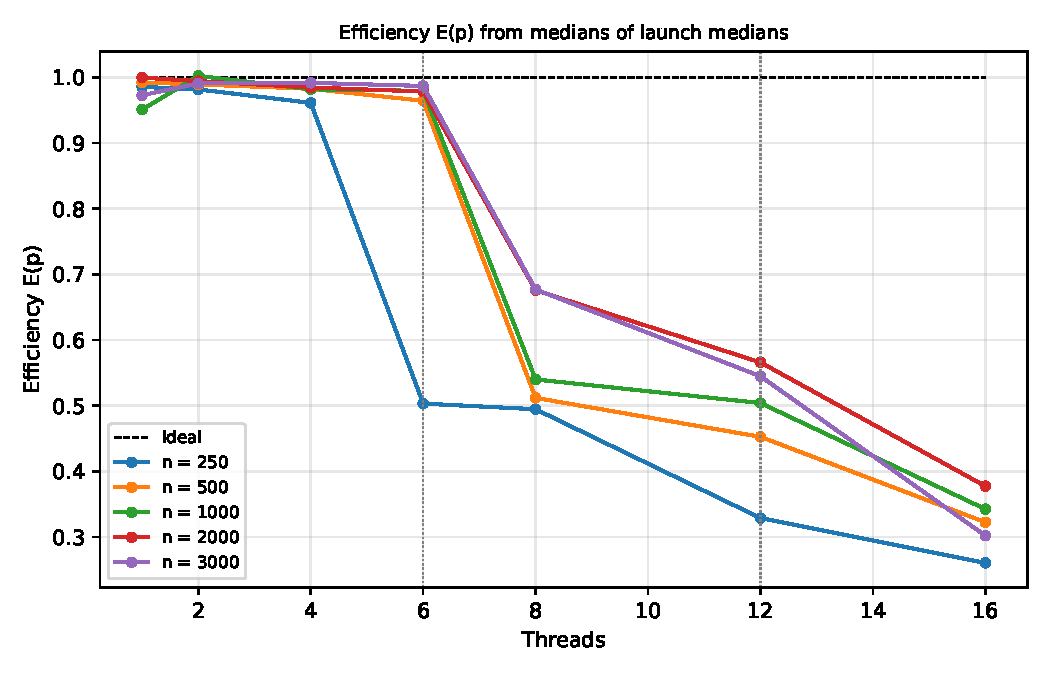
\includegraphics[width=0.75\linewidth]{figs/fig_efficiency_launches.pdf}
\caption{Parallel efficiency $E(p) = S(p)/p$ against the number of threads, with the ideal $E(p) = 1$.}\label{fig:eff}
\end{figure}

\subsection{Variation between launches}\label{sec:launches}

5 of the 120 launches are slow by the 10\,\% criterion: $n = 1000$ with 2 threads in launch 1 (+25\,\%, the 329.37\,ms result), $n = 1000$ with 6 threads in launch 3 (+26\,\%), $n = 1000$ with 4 threads in launch 3 (+16\,\%), $n = 500$ with 6 threads in launch 1 (+17\,\%) and $n = 250$ with 4 threads in launch 2 (+90\,\%, a 4.2\,ms run). For $n = 250$ the deviations go in both directions: one 6-thread launch is 47\,\% \emph{faster} than the other two. No launch with $n \ge 2000$ is more than 3.5\,\% away from the summary of its configuration.

Compared with launch 1 alone, which was the basis of the first version of this study, the summary medians change by less than 3\,\% in 38 of the 40 configurations. The two exceptions are $n = 1000$ with 2 threads ($-19.7$\,\%, so $S(2)$ rises from 1.63 to 2.00) and $n = 500$ with 6 threads ($-14.6$\,\%, so $S(6)$ rises from 4.94 to 5.79), both of which were slow launches in launch 1.

\subsection{Cost of the parallel machinery (one thread)}

\begin{table}[H]
\centering\small
\caption{Parallel implementation with one thread against the sequential baseline (summary medians).}\label{tab:onethread}
\begin{tabular}{@{}rrrr@{}}
\toprule
$n$ & Sequential (ms) & Parallel, 1 thread (ms) & Difference \\
\midrule
250 & 8.43 & 8.56 & +1.5\,\% \\
500 & 66.02 & 66.53 & +0.8\,\% \\
1000 & 530.12 & 557.51 & +5.2\,\% \\
2000 & 5354.17 & 5355.42 & +0.0\,\% \\
3000 & 18341.16 & 18854.49 & +2.8\,\% \\
\bottomrule
\end{tabular}
\end{table}

The one-thread parallel run is not faster than the baseline at any size, but the ranges of the launch medians of the two methods overlap at every size. For $n = 1000$ the follow-up measured a smaller difference, +0.9\,\% over 5 launches (Section~\ref{sec:followup}).

\subsection{Memory}

\begin{table}[H]
\centering\small
\caption{Memory per size, medians over the 3 launches. MB $= 10^6$ bytes, MiB $= 2^{20}$ bytes. Peak RSS is the peak resident set size of the whole JVM process.}\label{tab:memory}
\begin{tabular}{@{}rrrrrr@{}}
\toprule
$n$ & \shortstack{Estimated\\storage (MB)} & \shortstack{Live heap after\\GC, seq.\ (MB)} & \shortstack{Peak RSS,\\seq.\ (MiB)} & \shortstack{Peak RSS, par.\\1 thread (MiB)} & \shortstack{Peak RSS, par.\\16 threads (MiB)} \\
\midrule
250 & 1.5 & 3.31 & 140.6 & 139.8 & 156.8 \\
500 & 6 & 7.67 & 147.4 & 147.3 & 165.2 \\
1000 & 24 & 25.67 & 191.2 & 191.3 & 209.0 \\
2000 & 96 & 97.67 & 408.2 & 407.4 & 427.0 \\
3000 & 216 & 217.67 & 679.4 & 681.6 & 713.6 \\
\bottomrule
\end{tabular}
\end{table}

The live heap exceeds the estimated storage by about 1.7--1.8\,MB and does not depend on the thread count (parallel configurations of one size differ by about 10\,kB). The peak RSS grows with the thread count: from 1 to 16 threads it increases by 17.0, 17.9, 17.7, 19.6 and 32.0\,MiB for $n = 250$, 500, 1000, 2000 and 3000. The sequential and one-thread runs differ by at most 2.2\,MiB. Memory varies little between launches: the peak RSS of a configuration differs by at most 2.5\,MiB across its 3 launches.

\subsection{Correctness and limits}

All 120 launches passed the self-tests and the Freivalds check (0 failures), with status OK. For every size, all configurations of all launches produced the same checksum of $C$ (for example 60,758,230,789.87476 for $n = 3000$), consistent with bit-identical results. No multiplication reached the time or memory budget: the longest single sample was 18.88\,s ($n = 3000$, 1 thread) against the 240\,s limit. The largest size attempted, and also the largest tested, is $n = 3000$; no larger size was tried.

\subsection{Follow-up: $n = 1000$ over 35 JVM launches}\label{sec:followup}

All 35 launches passed the self-tests and the Freivalds check, with status OK, and all produced the same checksum of $C$ as the main study for $n = 1000$ (2,249,773,876.1382494). Table~\ref{tab:followup} summarises them and Figure~\ref{fig:launches} shows the median of every launch.

\begin{table}[H]
\centering\small
\caption{Follow-up for $n = 1000$: 5 JVM launches $\times$ 7 measured repetitions per configuration. Times in ms. $S$ is computed against the median of the launch medians of the follow-up's own sequential baseline (524.75\,ms).}\label{tab:followup}
\begin{tabular}{@{}llrrrc@{}}
\toprule
Configuration & CPUs & \shortstack{Median of\\launch medians} & \shortstack{Range of\\launch medians} & $S$ & \shortstack{Slow\\launches} \\
\midrule
Sequential & any & 524.75 & 523.09--614.65 & --- & 1 of 5 \\
Parallel, 1 thread & any & 529.51 & 524.02--614.90 & 0.99 & 1 of 5 \\
Parallel, 2 threads & any & 264.80 & 264.35--265.68 & 1.98 & 0 of 5 \\
Parallel, 4 threads & any & 132.94 & 132.52--157.35 & 3.95 & 1 of 5 \\
Parallel, 2 threads & 0,\,1 (two cores) & 266.46 & 262.83--329.85 & 1.97 & 1 of 5 \\
Parallel, 2 threads & 0,\,6 (one core) & 513.18 & 513.03--521.05 & 1.02 & 0 of 5 \\
Parallel, 1 thread & 0 & 537.38 & 529.28--565.67 & 0.98 & 0 of 5 \\
\bottomrule
\end{tabular}
\end{table}

\begin{figure}[htbp]
\centering
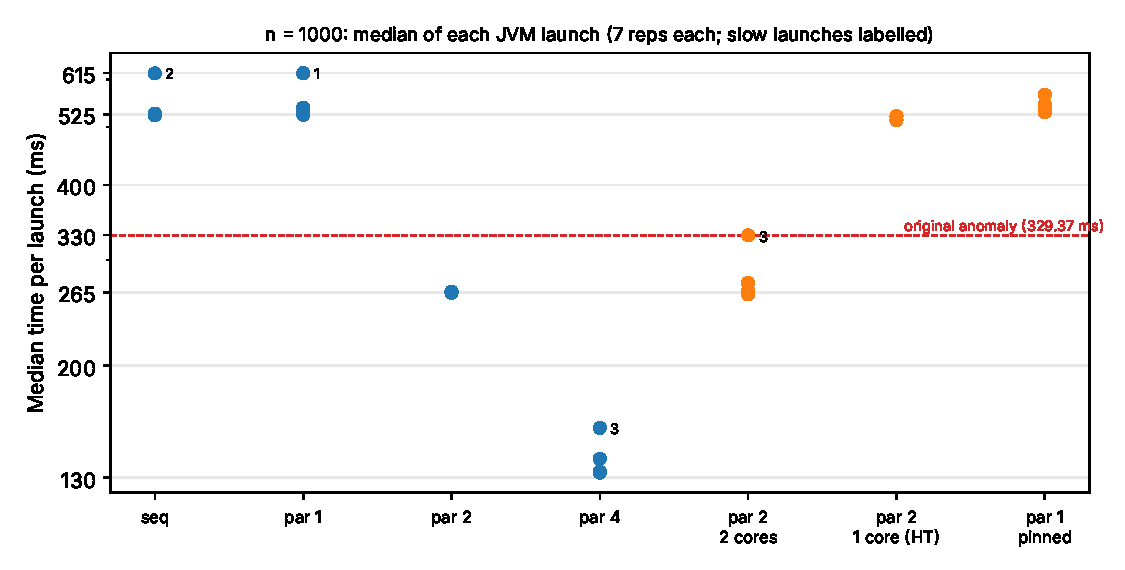
\includegraphics[width=0.85\linewidth]{figs/fig_n1000_launches.pdf}
\caption{Median of each JVM launch of the follow-up for $n = 1000$ (7 repetitions per launch; log scale). Blue: no affinity; orange: pinned with \code{taskset}. Slow launches are labelled with their launch number. Dashed line: the 2-thread median of launch 1 of the main study (329.37\,ms).}\label{fig:launches}
\end{figure}

\begin{itemize}
  \item \textbf{2 threads on two cores.} All 5 unpinned launches give 264.4--265.7\,ms ($S = 1.98$), and 4 of the 5 launches pinned to two physical cores give 262.8--274.6\,ms.
  \item \textbf{Slow launches.} 4 of the 35 launches are 16--24\,\% slower than the other launches of their configuration: sequential, parallel with 1 thread, parallel with 4 threads, and parallel with 2 threads pinned to two cores. The slow level is present from the first warm-up run and holds for all 10 runs of the launch, with a within-launch IQR of at most 4.65\,ms. The pinned slow launch took 329.85\,ms, within 0.2\,\% of the 329.37\,ms of launch 1 of the main study.
  \item \textbf{2 threads on one core.} With both threads on the two logical processors of one physical core the median is 513.18\,ms: 1.047 times the throughput of one pinned thread (537.38\,ms).
  \item \textbf{One thread.} The parallel code with one thread is 0.9\,\% slower than the sequential baseline (529.51 vs 524.75\,ms).
\end{itemize}

\subsection{Hyper-Threading test for $n = 2000$}\label{sec:ht2000}

\begin{table}[H]
\centering\small
\caption{Pinned placements for $n = 2000$, 3 launches each (7 repetitions per launch). Times in ms. Throughput relative to one pinned thread; $S$ against the sequential summary of Table~\ref{tab:runtime} (5354.17\,ms).}\label{tab:ht}
\begin{tabular}{@{}llrrrr@{}}
\toprule
Configuration & CPUs & \shortstack{Median of\\launch medians} & \shortstack{Range of\\launch medians} & \shortstack{Throughput vs\\one thread} & $S$ \\
\midrule
Parallel, 2 threads & 0,\,1 (two cores) & 2691.44 & 2685.72--2695.58 & 1.986 & 1.99 \\
Parallel, 2 threads & 0,\,6 (one core) & 4628.36 & 4625.24--4629.02 & 1.155 & 1.16 \\
Parallel, 1 thread & 0 & 5344.80 & 5341.98--5348.36 & 1.000 & 1.00 \\
\bottomrule
\end{tabular}
\end{table}

Two threads on two physical cores almost double the throughput (1.986). Two threads on the two logical processors of one core add 15.5\,\% (1.155). The three launches of each placement agree within 0.4\,\%, and none is slow.

\section{Discussion}

\subsection{Answer to the research question}

Parallel execution helps at every size tested, but it is efficient only up to the 6 physical cores. For $n \ge 500$, 6 threads give $S = 5.8$--$5.9$ ($E = 0.96$--$0.99$). Going to 12 threads, which puts a second thread on every core, shortens the median time by only 2.8\,\%, 13.6\,\% and 9.4\,\% for $n = 1000$, 2000 and 3000, at an efficiency of 0.50--0.57, and makes $n = 500$ slower. Using more threads than logical processors makes the runs slower. The smallest size gains less (best $S = 4.17$ for $n = 250$) and behaves irregularly.

\subsection{Hypotheses against the results}\label{sec:hyp}

\begin{itemize}
  \item \textbf{H1} (near-linear up to 6 threads): supported for $n \ge 500$ ($E(p) \ge 0.96$ for $p \le 6$). The low $S(2) = 1.63$ for $n = 1000$ in launch 1 was a slow launch; over 3 launches $E(2) = 1.00$.
  \item \textbf{H2} (efficiency falls between 6 and 12 threads): supported. $E(12) = 0.50$--$0.57$ for $n \ge 1000$ and $S$ never exceeds 6.8. It was also tested directly: a second thread on one physical core adds 4.7\,\% ($n = 1000$) and 15.5\,\% ($n = 2000$) of throughput.
  \item \textbf{H3} (no gain beyond the logical processors): supported for $n \ge 500$, where 16 threads is 5--35\,\% slower than 12.
  \item \textbf{H4} (earlier saturation for small $n$): supported. The speedup stops at about 4 for $n = 250$; for $n = 500$ the best configuration is 6 threads ($S = 5.79$) and 12 threads no longer helps, while for $n \ge 1000$ the best is 12 threads.
  \item \textbf{H5} (small one-thread penalty): supported. The difference is 0.0--2.8\,\% except for $n = 1000$ (+5.2\,\% over the 3 launches of the main study, +0.9\,\% over the 5 launches of the follow-up), and the launch ranges of the two methods overlap at every size.
\end{itemize}

\subsection{Explanations and the evidence for them}

\paragraph{Up to 6 threads.} The rows are independent, the chunks differ by at most one row, nothing is shared for writing and the serial part is negligible, so a near-linear speedup is expected. The measured efficiency shows no sign of a memory-bandwidth limit up to 6 threads for $n \ge 500$.

\paragraph{Between 6 and 12 threads.} With 12 threads every physical core runs two threads that share its execution resources~\cite{marr}. Two independent measurements agree on how much a second thread on a core adds. From the scaling runs, $S(12)/S(6)$ is 1.029 for $n = 1000$ and 1.157 for $n = 2000$. From the pinned runs, two threads on one core give 1.047 ($n = 1000$) and 1.155 ($n = 2000$) times the throughput of one thread on that core. The agreement for $n = 2000$ (1.157 vs 1.155) is especially close. For $n = 3000$, $S(12)/S(6) = 1.104$ is consistent with the same explanation but was not tested with pinning. Why the second thread adds more for $n = 2000$ than for $n = 1000$ was not investigated.

\paragraph{8 threads.} A simple check also fits the slow 8-thread runs. Let $r = S(12)/12$ be the speed of a thread that shares a core relative to a thread running alone ($r = 0.545$ for $n = 3000$). With 8 threads on 6 cores, two cores must host two threads each. With static chunks, a thread that shares a core needs $T_{\mathrm{seq}}/(8r) = 4.21$\,s, whereas a perfect redistribution of the work would take 2.97\,s; the observed 3.39\,s lies between the two. The same bracket holds for $n = 2000$ (855--1183\,ms, observed 990\,ms) and $n = 1000$ (88--131\,ms, observed 123\,ms). This is a consistency check built on assumptions about where the operating system places the threads, not a test.

\paragraph{Oversubscription (hypothesis).} With 16 equal static chunks on 12 logical processors, some threads must wait for others, the operating system has to time-share the cores and the static partition cannot rebalance the work. The loss of 10--35\,\% for $n \ge 1000$ is consistent with this, but the data cannot separate scheduling, context-switch and cache effects.

\paragraph{Slow launches.} The $S = 1.63$ result of launch 1 is not a property of the 2-thread configuration: launches 2 and 3 and all 5 unpinned follow-up launches give $S \approx 2.0$. It is not caused by both threads landing on one physical core either, because that placement, tested directly, takes 513\,ms, far slower than 329\,ms. Instead, a JVM launch can settle into a slow state that lasts for the whole launch: 4 of the 35 follow-up launches and 5 of the 120 launches of the main study were 16--26\,\% slower than the other launches of their configuration (ignoring the 4\,ms runs of $n = 250$), from the first warm-up run to the last repetition. It occurred with and without affinity and with 1, 2, 4 and 6 threads, and also in the sequential baseline, so it does not depend on the parallel code. It was seen only for $n = 500$ and $n = 1000$; for $n \ge 2000$ every launch lies within 3.5\,\% of its summary. Its cause was not tested. Plausible candidates, which would produce a per-launch rather than per-repetition effect, are a different JIT compilation of the kernel or a different placement of the arrays in memory; neither was measured.

\paragraph{Cost of the one-thread run.} Handing one task to a pool thread does not cost time proportional to $n^3$, and the difference to the baseline does not grow with $n$ (+0.0\,\% for $n = 2000$). For $n = 1000$ it changed between sessions (+5.2\,\% here, +0.9\,\% in the follow-up), so it is best read as launch variation rather than as a fixed cost of the pool.

\paragraph{No evidence of superlinear speedup.} The only value above the ideal is $E = 1.002$ ($n = 1000$, 2 threads), 0.2\,\% above 1, smaller than the 1.6\,\% range of the sequential launch medians at that size. We treat it as a measurement effect.

\subsection{Limitations}

\begin{itemize}
  \item One machine, one evening. Launch 1 and launches 2--3 were run in two sessions of the same day, and 3 launches per configuration only roughly estimate the launch-to-launch variation; the frequency of slow launches (about 4\,\% in the main study, 11\,\% in the follow-up) is an approximate figure.
  \item With 3 launches, one slow launch still moves the median only if a second launch is also slow, but the range of launch medians in Table~\ref{tab:runtime} is sensitive to single launches.
  \item No monitoring of CPU frequency or turbo, no per-thread timings, no hardware counters and no JIT logs. The explanations about oversubscription, the 8-thread runs and the cause of the slow launches are therefore hypotheses. The core-sharing explanation was tested only for 2 threads and $n = 1000$ and 2000. With \code{taskset} the whole JVM, including its JIT and GC threads, was restricted to the pinned CPUs.
  \item Only one algorithm (i-k-j) with static row partitioning and \code{double} values was tested. Dynamic scheduling, blocked kernels and other numeric types may behave differently.
  \item Sizes stop at $n = 3000$, and only the thread counts 1, 2, 4, 6, 8, 12 and 16 were measured.
\end{itemize}

\section{Conclusions}

Within the tested scope (one 6-core, 12-thread CPU, OpenJDK 21, the i-k-j kernel with static row partitioning, 64-bit values, $n = 250$ to $3000$, 3 JVM launches per configuration), the study establishes the following.
\begin{itemize}
  \item Splitting the rows of $C$ among threads gives correct, bit-identical results and a nearly linear speedup up to the 6 physical cores for $n \ge 500$ ($E = 0.96$--$0.99$).
  \item The shortest times are obtained with 12 threads for $n \ge 1000$, but they improve on 6 threads by only 2.8--13.6\,\%. The largest speedup is 6.79 ($n = 2000$, 12 threads). For $n = 500$ the best is 6 threads.
  \item A second thread on a physical core adds little: 4.7\,\% of throughput for $n = 1000$ and 15.5\,\% for $n = 2000$, measured directly with pinned threads and matching $S(12)/S(6)$.
  \item With static chunks, 8 threads are slower than 6 (by 9--41\,\% for $n \ge 500$) and 16 threads are slower than 12 (by 5--35\,\% for $n \ge 500$).
  \item The smallest size saturates at $S \approx 4$ and is irregular between launches.
  \item The parallel code with one thread costs 0--3\,\% against the sequential baseline, with a variable value for $n = 1000$. The live heap does not depend on the thread count, while the peak resident memory grows by 17--32\,MiB from 1 to 16 threads.
  \item JVM launches of the same configuration can differ by 16--26\,\% for their whole duration, seen here for $n = 500$ and 1000. A single launch per configuration is therefore not enough: in the first version of this study, two of the 40 results (including the anomalous $S = 1.63$) came from such launches.
\end{itemize}

\paragraph{Left unresolved.} The cause of the slow launches (a test would log JIT compilation with \code{-XX:+PrintCompilation} and record the array addresses or use pre-touched, aligned memory) and why they appear only for the middle sizes; why the second thread on a core helps more for $n = 2000$ than for $n = 1000$; the core-sharing test for $n = 3000$ and for more than 2 threads; and whether dynamic scheduling or a blocked kernel would change the picture beyond 6 threads.

\section{References and materials}


\renewcommand{\refname}{References}
\begingroup
\renewcommand{\section}[2]{}
\begin{thebibliography}{9}\small
\bibitem{gustafson} J.~L. Gustafson, ``Reevaluating Amdahl's law,'' \emph{Commun. ACM}, vol.~31, no.~5, pp.~532--533, 1988. [Online]. Available: \url{https://users.cs.utah.edu/~hari/teaching/paralg/Gustafson88.pdf}
\bibitem{goto} K.~Goto and R.~A. van de Geijn, ``Anatomy of high-performance matrix multiplication,'' \emph{ACM Trans. Math. Softw.}, vol.~34, no.~3, art.~12, 2008. [Online]. Available: \url{https://cs.utexas.edu/~flame/pubs/GotoTOMS.pdf}
\bibitem{roofline} S.~Williams, A.~Waterman and D.~Patterson, ``Roofline: an insightful visual performance model for multicore architectures,'' \emph{Commun. ACM}, vol.~52, no.~4, pp.~65--76, 2009. [Online]. Available: \url{https://escholarship.org/content/qt78h8v7mr/qt78h8v7mr.pdf}
\bibitem{marr} D.~T. Marr \emph{et al.}, ``Hyper-Threading technology architecture and microarchitecture,'' \emph{Intel Technology Journal}, vol.~6, no.~1, 2002. [Online]. Available: \url{https://www.intel.com/content/dam/www/public/us/en/documents/research/2002-vol06-iss-1-intel-technology-journal.pdf}
\bibitem{freivalds} R.~Freivalds, ``Probabilistic machines can use less running time,'' in \emph{Information Processing 77, Proc. IFIP Congress 1977}, Amsterdam, The Netherlands: North-Holland, 1977.
\end{thebibliography}
\endgroup

\subsection*{Reproducibility materials}

\begin{itemize}
  \item \textbf{Repository for this assignment:} \url{https://github.com/Pancrasi0/-Big-Data-Individual-Assignment-III}.
  \item \textbf{Reused code:} the \code{ikj\_reorder} kernel and the input generator of Assignment~2, repository \href{https://github.com/Pancrasi0/Big-Data-Individual-Assignment-II}{Big-Data-Individual-Assignment-II}, commit \url{3408430bc67a82561e8619e546ce9e351c82dee0}.
  \item \textbf{Contents of the repository:} Java source code, a README with the exact build and run commands, the scripts \code{build.sh}, \code{run\_all.sh}, \code{analyze.py}, \code{run\_n1000.sh}, \code{analyze\_n1000.py}, \code{run\_rigor.py} and \code{analyze\_rigor.py}, and all raw measurements with their \code{environment.txt} files: launch 1 of the main study in \code{results/}; the $n = 1000$ follow-up in \code{results\_n1000/} (one directory per experiment and launch, with \code{lscpu\_e.txt}, the CPU pairs used and the run log); launches 2 and 3 and the $n = 2000$ Hyper-Threading test in \code{results\_rigor/}, whose \code{analysis/} directory holds the combined summaries and the figures of this report.
  \item \textbf{To reproduce:} \code{bash scripts/build.sh}; then \code{bash scripts/run\_all.sh} (launch 1), \code{python3 scripts/run\_rigor.py} (launches 2 and 3 and the Hyper-Threading test) and \code{python3 scripts/analyze\_rigor.py} (all tables and Figures 1--3); for the follow-up, \code{bash scripts/run\_n1000.sh} and \code{python3 scripts/analyze\_n1000.py results\_n1000}. The inputs are regenerated from the seeds 42 and 43; nothing needs to be downloaded.
\end{itemize}

\subsection*{Use of generative AI}

Tool: Claude (Anthropic). Purpose: writing the benchmark code and analysis scripts, designing the $n = 1000$ follow-up, the extra launches and the Hyper-Threading test and their scripts, and drafting this report and its \LaTeX{} version from the measurements. Affected parts: the benchmark code, the scripts and the text of the report. The author reviewed the code, ran all measurements on their own machine and is responsible for the results, their interpretation and the conclusions.

\end{document}
